\documentclass[hidelinks,12pt]{article}
\usepackage[left=0.25cm,top=1cm,right=0.25cm,bottom=1cm]{geometry}
%\usepackage[landscape]{geometry}
\textwidth = 20cm
\hoffset = -1cm
\usepackage[utf8]{inputenc}
\usepackage[spanish,es-tabla, es-lcroman]{babel}
\usepackage[autostyle,spanish=mexican]{csquotes}
\usepackage[tbtags]{amsmath}
\usepackage{nccmath}
\usepackage{amsthm}
\usepackage{amssymb}
\usepackage{mathrsfs}
\usepackage{graphicx}
\usepackage{subfig}
\usepackage{caption}
%\usepackage{subcaption}
\usepackage{standalone}
\usepackage[outdir=./Imagenes/]{epstopdf}
\usepackage{siunitx}
\usepackage{physics}
\usepackage{color}
\usepackage{float}
\usepackage{hyperref}
\usepackage{multicol}
\usepackage{multirow}
%\usepackage{milista}
\usepackage{anyfontsize}
\usepackage{anysize}
%\usepackage{enumerate}
\usepackage[shortlabels]{enumitem}
\usepackage{capt-of}
\usepackage{bm}
\usepackage{mdframed}
\usepackage{relsize}
\usepackage{placeins}
\usepackage{empheq}
\usepackage{cancel}
\usepackage{pdfpages}
\usepackage{wrapfig}
\usepackage[flushleft]{threeparttable}
\usepackage{makecell}
\usepackage{fancyhdr}
\usepackage{tikz}
\usepackage{bigints}
\usepackage{menukeys}
\usepackage{tcolorbox}
\tcbuselibrary{breakable}
\usepackage{scalerel}
\usepackage{pgfplots}
\usepackage{pdflscape}
\pgfplotsset{compat=1.16}
\spanishdecimal{.}
\renewcommand{\baselinestretch}{1.5} 
\renewcommand\labelenumii{\theenumi.{\arabic{enumii}})}

\newcommand{\python}{\texttt{python}}
\newcommand{\textoazul}[1]{\textcolor{blue}{#1}}
\newcommand{\azulfuerte}[1]{\textcolor{blue}{\textbf{#1}}}
\newcommand{\funcionazul}[1]{\textcolor{blue}{\textbf{\texttt{#1}}}}

\newcommand{\pderivada}[1]{\ensuremath{{#1}^{\prime}}}
\newcommand{\sderivada}[1]{\ensuremath{{#1}^{\prime \prime}}}
\newcommand{\tderivada}[1]{\ensuremath{{#1}^{\prime \prime \prime}}}
\newcommand{\nderivada}[2]{\ensuremath{{#1}^{(#2)}}}


\newtheorem{defi}{{\it Definición}}[section]
\newtheorem{teo}{{\it Teorema}}[section]
\newtheorem{ejemplo}{{\it Ejemplo}}[section]
\newtheorem{propiedad}{{\it Propiedad}}[section]
\newtheorem{lema}{{\it Lema}}[section]
\newtheorem{cor}{Corolario}
\newtheorem{ejer}{Ejercicio}[section]

\newlist{milista}{enumerate}{2}
\setlist[milista,1]{label=\arabic*)}
\setlist[milista,2]{label=\arabic{milistai}.\arabic*)}
\newlength{\depthofsumsign}
\setlength{\depthofsumsign}{\depthof{$\sum$}}
\newcommand{\nsum}[1][1.4]{% only for \displaystyle
    \mathop{%
        \raisebox
            {-#1\depthofsumsign+1\depthofsumsign}
            {\scalebox
                {#1}
                {$\displaystyle\sum$}%
            }
    }
}
\def\scaleint#1{\vcenter{\hbox{\scaleto[3ex]{\displaystyle\int}{#1}}}}
\def\scaleoint#1{\vcenter{\hbox{\scaleto[3ex]{\displaystyle\oint}{#1}}}}
\def\scaleiiint#1{\vcenter{\hbox{\scaleto[3ex]{\displaystyle\iiint}{#1}}}}
\def\bs{\mkern-12mu}

\newcommand{\Cancel}[2][black]{{\color{#1}\cancel{\color{black}#2}}}


\usepackage{minted}

\author{M. en C. Gustavo Contreras Mayén. \texttt{gux7avo@ciencias.unam.mx}}
\title{Lista de ejercicios a cuenta para el Tema 1 \\ {\large Curso Física Computacional}}
\date{ }
\begin{document}

\maketitle
\fontsize{14}{14}\selectfont

\begin{enumerate}
\item Para el ejercicio del estudio de la velocidad en la bicicleta: hay que implementar el código en \python, considerando los valores $C = 0.5$ y $A=0.33$. De tal manera que al obtener la gráfica de la solución, debes de presentar una figura con el siguiente resultado:
\begin{figure}[H]
	\centering
	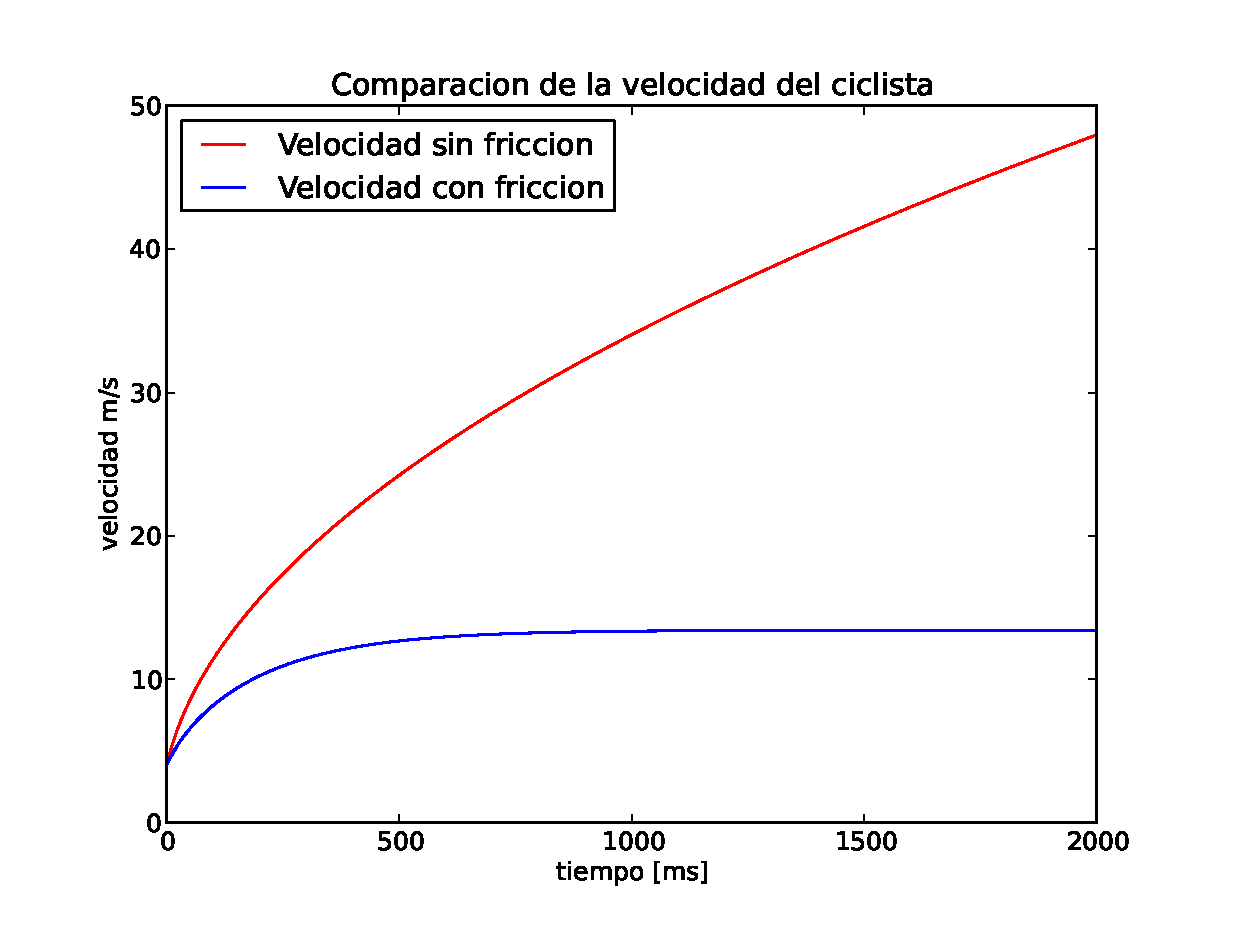
\includegraphics[scale=0.475]{Imagenes/EjerBicicleta02.eps}
\end{figure}
\item El número $\ln \, 2$ se puede calcular de la serie:
\begin{align*}
\ln 2 = 1 - \dfrac{1}{2} + \dfrac{1}{3} -\dfrac{1}{4} + \ldots
\end{align*}
Se sabe del análisis que esta serie converge y que la magnitud del error en cualquier suma parcial es menor que la magnitud del primer término despreciado. Estima el número de términos que se requerirían para calcular $\ln 2$ con $10$ decimales.
\item El 25 de febrero de 1991, durante la guerra del Golfo, una batería de misiles Patriot americanos en Dharan (Arabia Saudita) no lograron interceptar un misil Scud iraquí. Murieron 28 soldados americanos.
\par
La causa: los errores numéricos por utilizar truncado en lugar de redondeo en el sistema que calcula el momento exacto en que debe ser lanzado el misil. Las computadoras de los Patriot que han de seguir la trayectoria del misil Scud, la predicen punto a punto en función de su velocidad conocida y del momento en que fue detectado por última vez en el radar.
\par
La velocidad es un número real. El tiempo es una magnitud real pero el sistema la calculaba mediante un reloj interno que contaba décimas de segundo, por lo que representaban el tiempo como una variable entera Cuanto más tiempo lleva el sistema funcionando más grande es el entero que representa el tiempo. Las computadoras del Patriot almacenan los números reales representados en punto flotante con una mantisa de $24$ bits. Para convertir el tiempo entero en un número real se multiplica éste por $1/10$, y se trunca el resultado (en lugar de redondearlo). El número $1/10$ se almacenaba truncado a $24$ bits.
\par
El pequeño error debido al truncado, se hace grande cuando se multiplica por un número (entero) grande, y puede conducir a un error significativo. La batería de los Patriot llevaba en funcionamiento más de $100$ horas, por lo que el tiempo entero era un número muy grande y el número real resultante tendrá un error cercano a $0.34$ segundos. \textbf{Explica a detalle qué fue lo que ocurrió}.
\end{enumerate}

\end{document}